\chapter{Design}
\todo{short introduction to what will be addressed in this chapter}
This chapter describes the design process for this project. Initially, the concept of the product is presented...

\section{Concept}
The concept of the product is to be able to apply voice effects in real-time without having to turn to a panel or having someone do it for you. 

A thing most singers almost always have available are their hands. Therefore a device controlled by the hands movements seems the obvious choice.

The device will implement a gyroscope to sense the movements of the hand.

The device then needs to be told that an effect has been initiated. This is done by connecting the thumb to the finger in control of the desired effect.


\begin{itemize}
\item Harmonising: This will be controlled by turning the hand while having thumb and a finger pressed together, like turning a knob or volume control.
\item Pitch: This will be controlled by lifting or lowering the hand while having thumb and a finger pressed together, like pulling a slider up or down.
\end{itemize}

\section{Storyboard}

To understand the concept and how it would work in a real scenario a storyboard was created to explain how, what and where to use the product. this storyboard was part of the proof of concept that together with the initial sketches would explain the idea better.\\

\begin{minipage}{\linewidth}% to keep image and caption on one page
\makebox[\linewidth]{%        to center the image
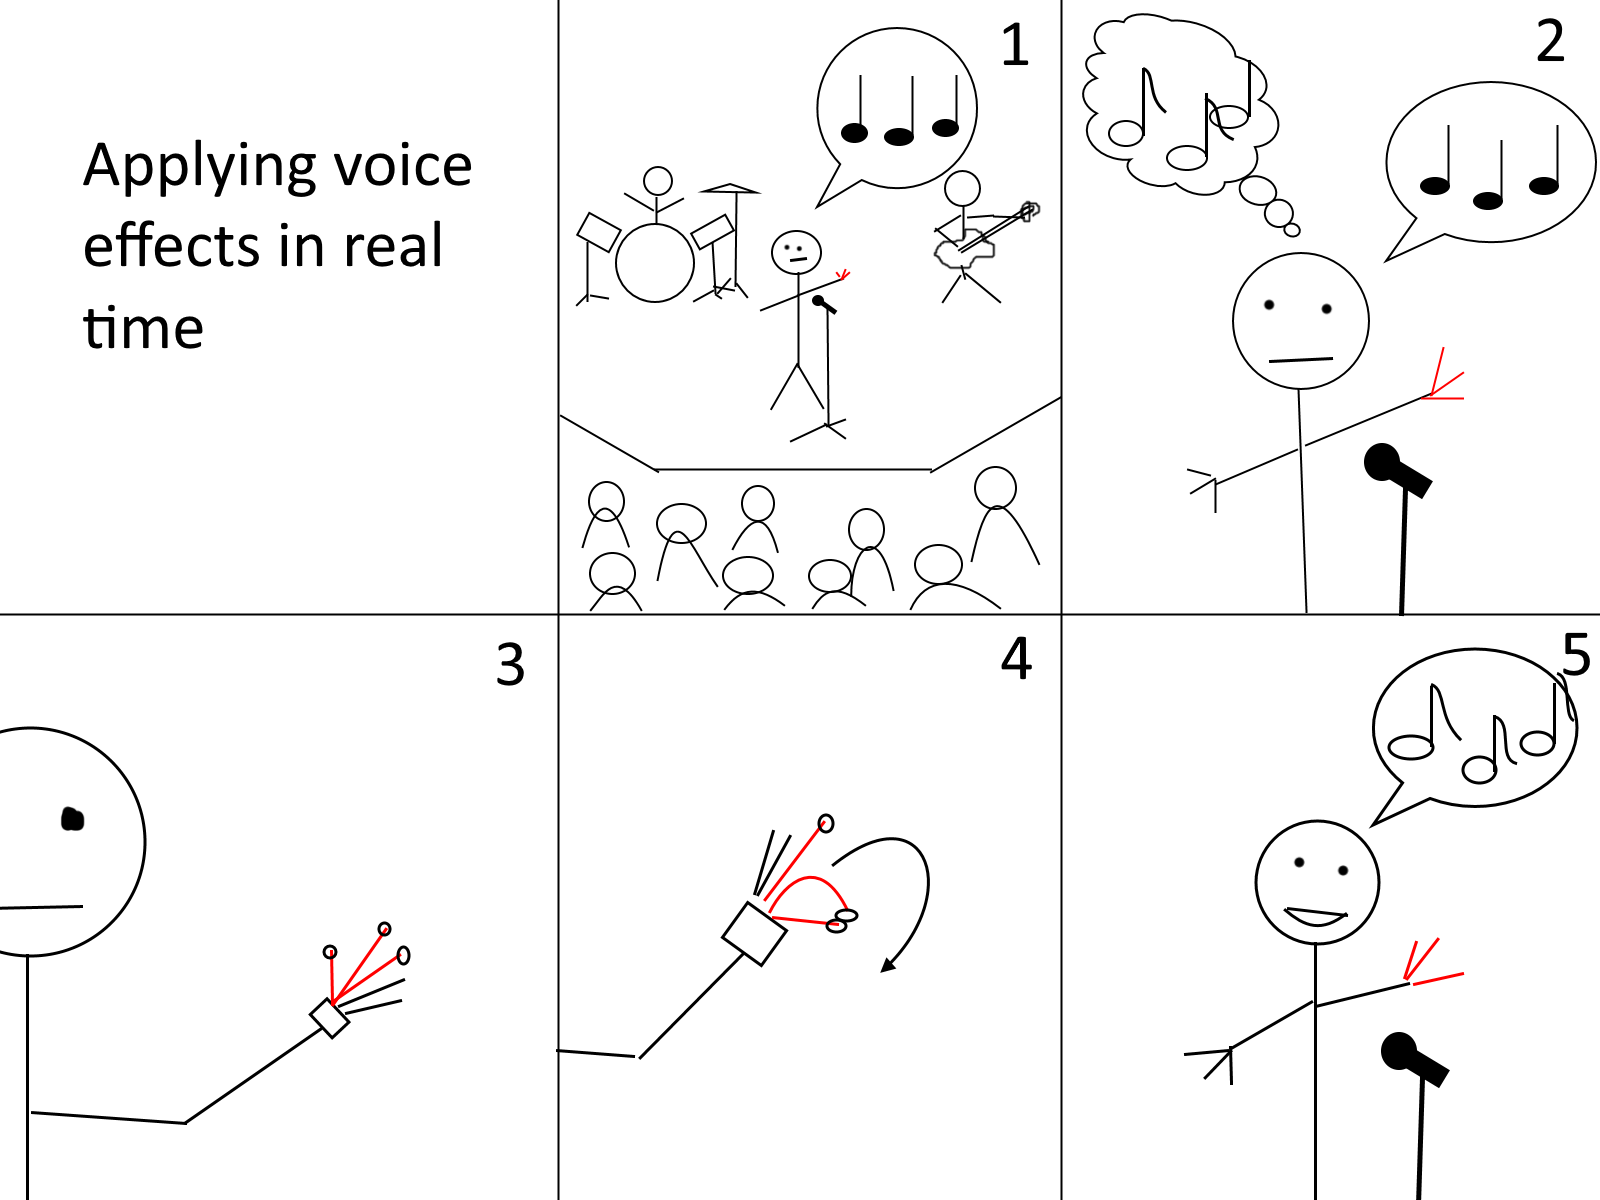
\includegraphics[keepaspectratio=true,scale=0.3]{Storyboard2}}
\captionof{figure}{The Storyboard}}\label{Storyboard}
\end{minipage}\\

In the first frame a band is shown playing a concert on a stage, with the lead singer singing. The seond frame shows the lead singer singing, but wanting to sound different. In the third frame the device is shown on the singer's hand. Fourth frame illustrates the singer performing a gesture to apply the desired effect. The final frame then shows the singer sounding how they wanted to sound.

\section{Sketching and Testing}

The initial sketches and the first concrete design of the device have copper foil on thumb, index finger and middle finger, see figure \ref{Sketch1}. When pressing the index or middle finger together with the thumb, a connection is made in the system that activates the assigned effect. \\

\begin{minipage}{\linewidth}% to keep image and caption on one page
\makebox[\linewidth]{%        to center the image
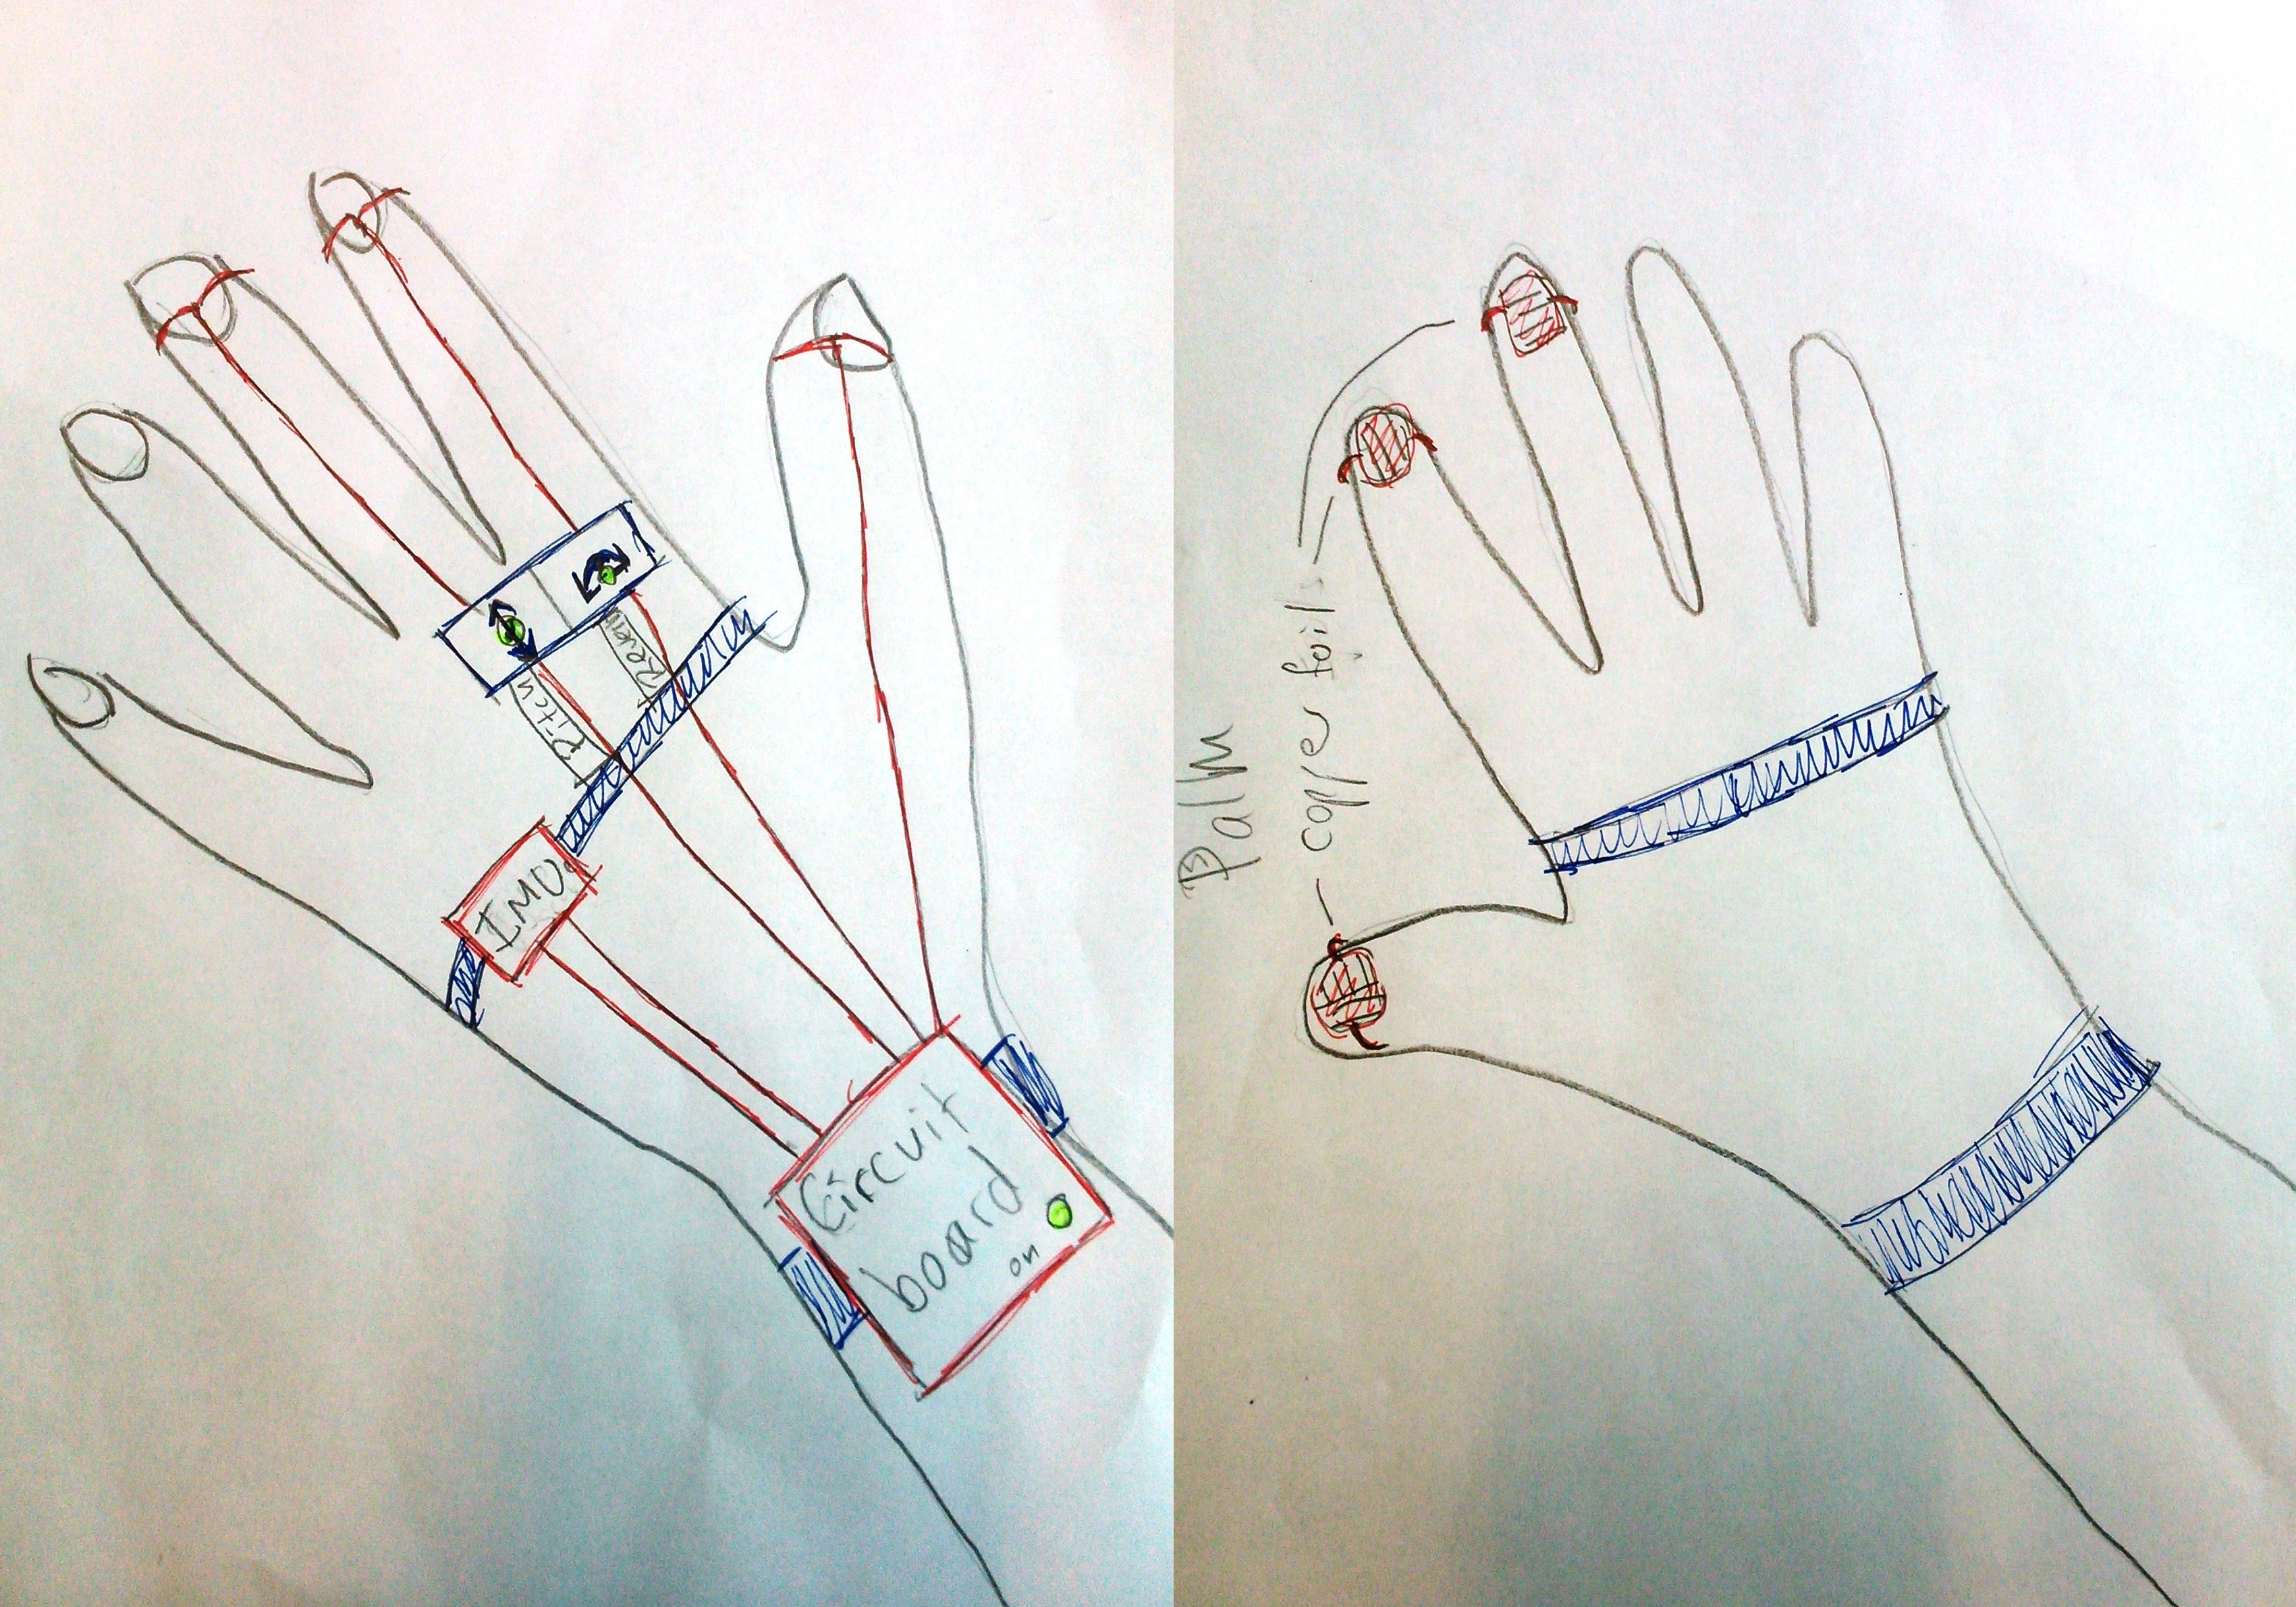
\includegraphics[keepaspectratio=true,scale=0.1]{Sketch1}}
\captionof{figure}{Two sketches showing idea of the system}}\label{Sketch1}
\end{minipage}\\

On the knuckles there are illustrations of the gestures, that you are supposed to do to manipulate the effects. Beneath those are small labels with the name of the effect. In this design reverb is used instead of harmonising. This was later changed, since reverb is not manipulated quite as much as harmonising.

The sensor is attached to the hand by a velcro strip, as is the circuit board. \\

A quick informal test with three participants was conducted and they were told what the drawing was supposed to be and what it should do. They then had to figure out based on the sketch how to do those things.
From this test, a few key things were learned:
 
\begin{itemize}
	\item They all had difficulty figuring out how to get to the activate stage. None of them connected their fingers.
	\item Most eventually figured out which type of gesture in general had to be done, but only after some trial and error
	\item They all found out which finger created which effect
\end{itemize}

Based on that the next focus was on creating some feedforward and perceived affordance that tells the user, that to activate the glove you need to connect two fingers.

The second sketch changed the illustrations since people had a hard time immediately recognising the correct gestures with the old ones, as seen in figure \ref{Sketch2}.\\

\begin{minipage}{\linewidth}% to keep image and caption on one page
\makebox[\linewidth]{%        to center the image
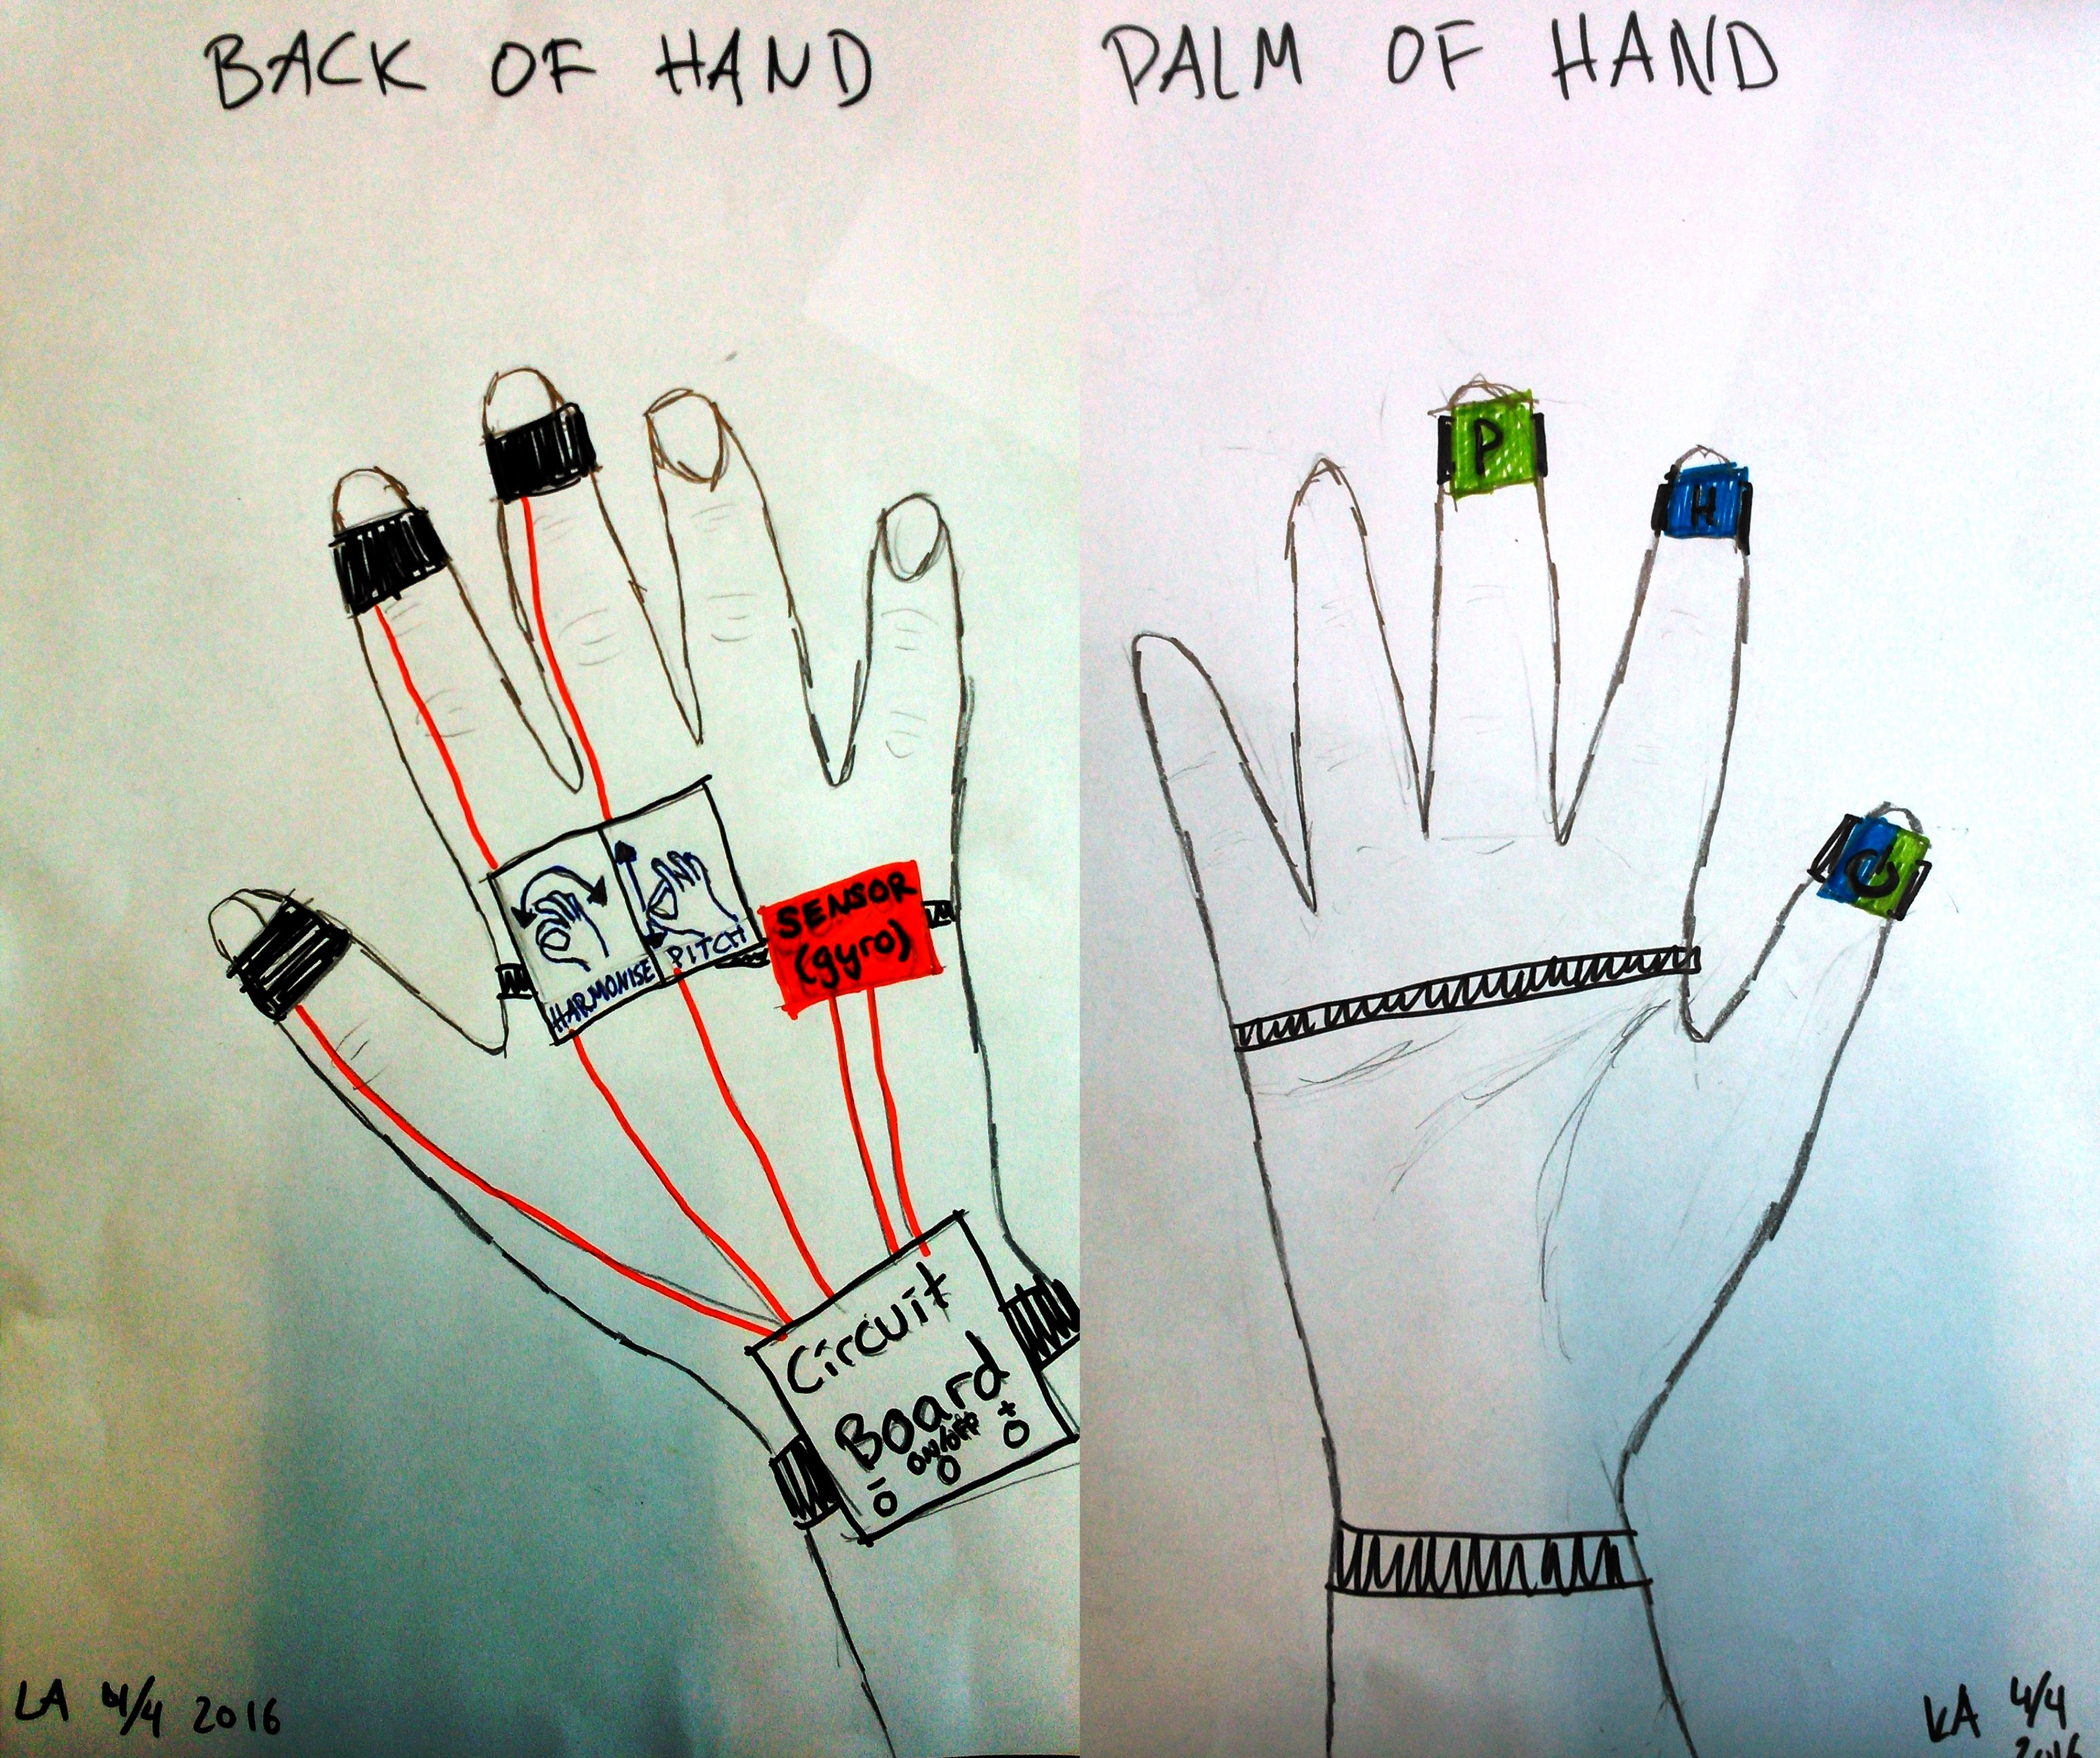
\includegraphics[keepaspectratio=true,scale=0.1]{Sketch2}}
\captionof{figure}{Second set of sketches after some changes}}\label{Sketch2}
\end{minipage}\\

Colour was also added to the copper foil, a different one on the index and middle finger and then both on the thumb. This was done to create perceived affordance between the fingers and thumb.

LEDs were added on the circuit board to create some feedback for the actions. The middle LED showing if the system was on or off. The two other LEDs showing an increase or decrease in the effect, with a minus and a plus sign.\\

A quick informal test was done with two participants with the revised sketch. Now there was a better indication that they needed to connect two fingers, but not anything that indicated that they needed to stay connected.
Additional results from the test:

\begin{itemize}
	\item One suggested that instead of the on/off LED, maybe a connected/not connected LED.
	\item The arrows were found to be confusing for one tester.
	\item Another tester easily understood the pitch action but was a bit confused with the placement of the arrow on the harmonise action.
	\item One tester thought tht the dual colour on the thumb suggested that both actions could be done at the same time.
	\item The plus and minus LEDs confused one tester, but this could also be because the drawing was unclear.
\end{itemize} 

\section{Lo-Fi}

Based on the previous test, a new design iteration of the glove was made, now also in the form of a lo-fi model, as seen in figure \ref{LoFiHand}. This lo-fi was created in order to make a mental model test. The desire was to both get some feedback on the general design, but also to weigh the feedback against an affordance scheme.

\begin{minipage}{\linewidth}% to keep image and caption on one page
\makebox[\linewidth]{%        to center the image
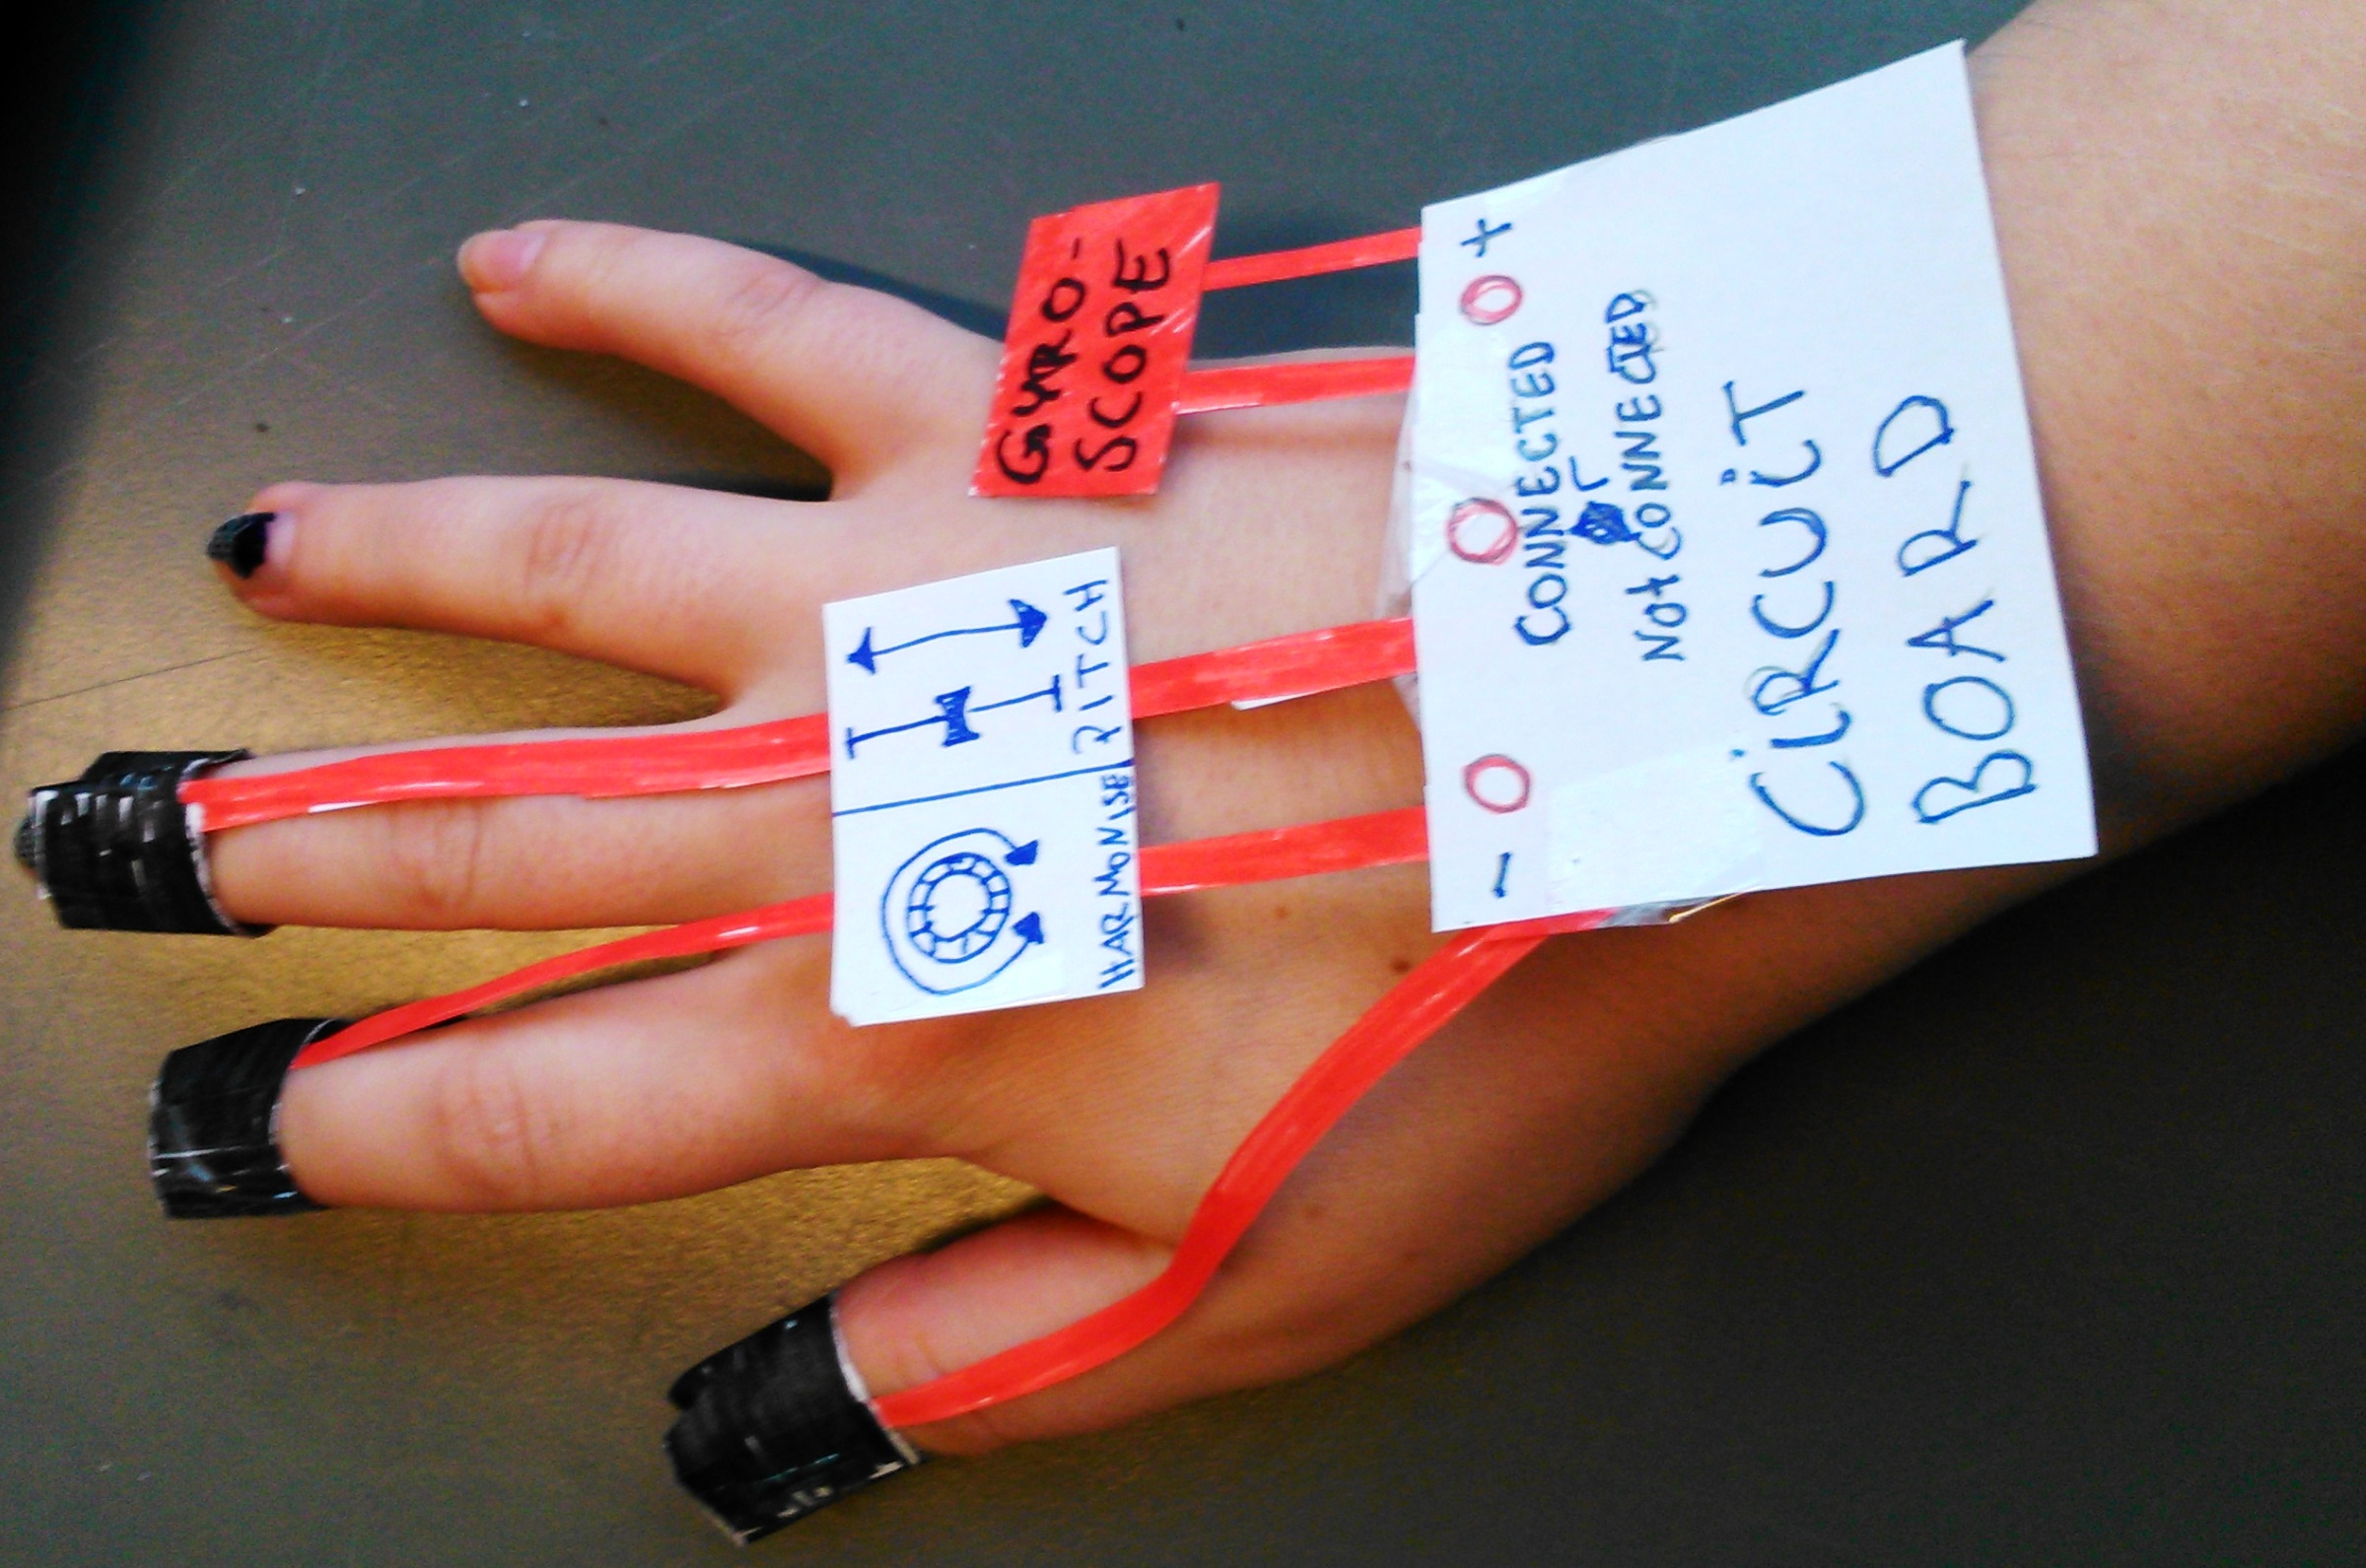
\includegraphics[keepaspectratio=true,scale=0.1]{LoFiHand}}
\captionof{figure}{The Lo-fi of the system}}\label{LoFiHand}
\end{minipage}\\

\subsection{Affordance Scheme}
The affordance scheme is separated into three categories: perceived affordance, feedforward, and feedback. Perceived affordance is the perception that something is interactable, e.g. a user would assume a button can be pressed no matter what state the system is in. Feedforward is what is expected to happen after a certain action, e.g. after pressing the "On" button, the system will turn On. Finally, feedback is what the system does to indicate an action has taken place, e.g. after pressing the "On" button, a display lights up and says "Turning On".

The following table shows the affordance scheme for the current lo-fi design, as seen in figure \ref{LoFiHand}.

\begin{center}
  \begin{tabular}{| c | c | c | c |}
    \hline
    \textbf{State} & \textbf{Perceived Affordance} & \textbf{Feedforward} & \textbf{Feedback} \\ \hline
    \textbf{Inactive} & It is a wearable glove & & All LEDs are OFF \\ \hline
    \textbf{Active} &  & Connect fingers + perform gesture on labels = effect change & "Connected" LED is ON \\ \hline        
    \textbf{Performing Gesture} &  & Connect fingers + perform gesture = effect change & Voice Changes and the plus and minus LEDs light accordingly \\ \hline
  \end{tabular}
\end{center}